\documentclass{standalone}

\usepackage{bm}
\usepackage{tikz}
\usepackage{tikz-3dplot}
\usepackage{tikzscale}
\usetikzlibrary{arrows,shapes,chains,matrix,positioning}
\usetikzlibrary{scopes,decorations,shadows,backgrounds,fit}
\usetikzlibrary{decorations.pathreplacing,calc,3d,patterns}
\usetikzlibrary{calc,decorations,decorations.pathreplacing}

\usepackage{amsmath}
\usepackage{amssymb}
\usepackage{amsthm}
\usepackage{amsfonts}

\tikzstyle{circ} = [draw, circle, fill=white!20, node distance=2cm,circular drop shadow, minimum height=1em]
\tikzstyle{block1} = [rectangle, draw, text width=14em, text centered, minimum height=4em, rounded corners]
\tikzstyle{block2} = [rectangle, draw, fill=blue!20, text width=2em, text centered, minimum height=2em]
\tikzstyle{block3} = [rectangle, draw, fill=green!20, text width=2em, text centered, minimum height=2em]

\begin{document}
    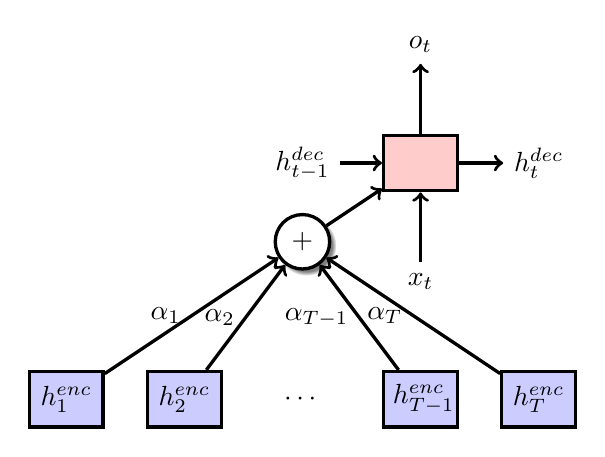
\begin{tikzpicture}[very thick]
        \node[] (a1) {$\cdots$};
        \node[block2, left of=a1, node distance=3.0cm] (a2) {$h_1^{enc}$};
        \node[block2, left of=a1, node distance=1.5cm] (a3) {$h_2^{enc}$};
        \node[block2, right of=a1, node distance=1.5cm] (a4) {$h_{T-1}^{enc}$};
        \node[block2, right of=a1, node distance=3.0cm] (a5) {$h_{T}^{enc}$};
        \node[block2, above of=a4, node distance=3.0cm, fill=red!20] (a6) {};
        \node[circ, above of=a1, node distance=2cm] (b1) {+};

        \node[right of=a6, node distance=1.5cm] (c1) {$h_t^{dec}$};
        \node[left of=a6, node distance=1.5cm] (c2) {$h_{t-1}^{dec}$};
        \node[above of=a6, node distance=1.5cm] (c3) {$o_t$};
        \node[below of=a6, node distance=1.5cm] (c4) {$x_t$};

        \draw[->] (a2) -- node[midway, left] {$\alpha_1$} (b1);
        \draw[->] (a3) -- node[midway, left] {$\alpha_2$} (b1);
        \draw[->] (a4) -- node[midway, left] {$\alpha_{T-1}$} (b1);
        \draw[->] (a5) -- node[midway, left] {$\alpha_T$} (b1);
        \draw[->] (b1) -- (a6);

        \draw[->] (a6) -- (c1);
        \draw[->] (c2) -- (a6);
        \draw[->] (a6) -- (c3);
        \draw[->] (c4) -- (a6);

    \end{tikzpicture}
\end{document}